\documentclass[12pt]{article}
%\usepackage{amsthm,amsmath,natbib}
\usepackage[top=2.5cm, bottom=3cm, left=2cm, right=2cm]{geometry}
\usepackage{amsthm,amsmath, color}
\usepackage{amsfonts}
\usepackage{graphicx}
\usepackage{latexsym,amsmath, color}
\usepackage{amsthm}
\usepackage[latin1]{inputenc}
\usepackage{times}
\usepackage[T1]{fontenc}
\usepackage{tikz-qtree}
\usepackage{tabularx}
\usepackage{dsfont}
\usepackage{algorithm}
\usepackage{algpseudocode}
\usepackage{listings}
\usepackage{longtable}
\usepackage{natbib}

\bibliographystyle{abbrvnat}
\setcitestyle{authoryear,open={(},close={)}}
\setlength\parindent{0pt}

\newcommand{\I}{\mathcal{I}}
\newcommand{\J}{\mathcal{J}}




\setlength{\parskip}{5pt}


%\startlocaldefs
\renewcommand{\theequation}{\thesection.\arabic{equation}}
\newcounter{thm}[section]
\newcounter{appen}
\renewcommand{\thethm}{\arabic{section}.\arabic{thm}}
\newtheorem{theor}[thm]{Theorem}
\newtheorem{cor}[thm]{Corollary}
\newtheorem{lem}[thm]{Lemma}
\newtheorem{proposition}[thm]{Proposition}
%\renewcommand{\theappen}{\thesection.\arabic{appen}}
\newtheorem{assumption}[appen]{Assumption}
\newtheorem{lemma}[appen]{Lemma}
\newtheorem{propa}[appen]{Proposition}
\newtheorem{hp}{Assumption}
\renewcommand{\thehp}{\Alph{hp}}
\def\esp{\mathbb{E}}
%\endlocaldefs


\begin{document}


\title{Bayesian non-parametric inference with monotonicity restrictions for discrete choice experiments}
\author{
	Remi Daviet \footnote{Corresponding author. Department of economics, University of Toronto; remi.daviet@mail.utoronto.ca} \quad and \quad
	William McCausland\footnote{Department of economics, Universit\'e de Montr\'eal}
}
\date{\today}


\maketitle

\begin{abstract}
	Insert abstract here
\smallskip


\end{abstract}

\quad

\textbf{Keywords:} Big Data, Discrete Choice experiments
%%%%%%%%%%%%%%%%%%%%%%%%

\newpage

\section{Products attributes and products classes}

Every product considered is represented by a point in the chosen attributes space. For instance, a mobile phone can be represented by a set of two attributes, the screen size and the color. Each attribute has a level. In our example, the screen size can have 3 levels $(Small, Medium \text{ or } Large)$ and the color can have 4 levels $(Black, White, Blue \text{ or } Other)$.  Considering this attributes space, two possible phones are phone 1 $(Large,Blue)$ and phone 2 $(Medium, White)$.

Products can be regrouped into classes. Classes are set of attributes commons to every product  belonging to the class. A class can be very simple, for instance the class $(\{Small\},any)$ which regroups all the phones with a small screen size, no matter the color. Classes can also be more complicated such as $(\{Small,Large\},\{White,Other\})$ which regroups phones of small or large screen size having a white or "other" color. Note that the $(\{Small\},any)$ class can be written $(\{Small\},\{ Black,White,Blue,Other\})$ and that the keyword "any" is just used for convenience. Finally, a class can specify a unique product in the attribute space, such as the class $(\{Large\},\{Blue\})$.

More formally, considering a product space with $L$ attributes, a product $x_m$ is represented by the vector of attributes $(x_{m1},x_{m2},\ldots,x_{mL})$. Each attribute $i$ can have $L_i$ possible levels. For instance, if the attribute $(1)$ "screen size" has $3$ possible levels $(Small, Medium \text{ or } Large)$, we write $L_1=3$. For the second attribute "Color" which has $4$ possible levels, we write $L_2=4$. The attributes levels attributed to a product $x_m$ are indicated by their corresponding number. For instance, if $Small$ and $Black$ are the first levels of their respective attributes, the phone will be represented by the vector $(x_{m1}=1,x_{m2}=1)$.

A class of product $\Lambda_k$ is represented by a Cartesian product of $L$ sets $(\Lambda_{k1},\Lambda_{k2},\ldots,\Lambda_{kL})$. Each $\Lambda_{ki}$ represents the set of possible levels for the attribute $i$ for a product in the class $k$. The levels belonging to $\Lambda_{ki}$ are called active levels. For instance, a class regrouping $Black$ phones with either $Medium \text{ or } Large$ screen size will be represented by $(\Lambda_{k1}=\{2,3\},\Lambda_{k2}=\{1\})$. When all the levels of an attribute are active, it means that this particular attribute does not matter when defining the class, and the attribute is defined as inactive. On the contrary, when only some levels are active, it means that the attribute is used as a criterion to select if a product is a member of the class, and the attribute is defined as active.

A product $x_m$ belongs to a class $\Lambda_k$ if and only if $ x_{m1} \in \Lambda_{k1},x_{m2} \in \Lambda_{k2},\ldots \text{ and } x_{mL} \in \Lambda_{kL}$. For convenience, we will use the notation $x_{m} \in \Lambda_{k}$ to indicate that the product $x_{m}$ is a member of the class $\Lambda_{k}$.

\section{Individual preferences}

We have a population of individuals, each one choosing a product within a set at a time $t$. The choice of an individual $n$ is done by maximizing a function $u(x,\psi)$ representing the preferences this individual over the set of available choices $X_{nt}$, where $\psi$ is some set of parameters. The choice maximizing the individual preferences is denoted $x^*$. The preferences for each individual are built by attributing some value to various classes of products. The value of a class can be positive or negative. For instance, at a time $t$ an individual $n$ attributes the value $\theta_{nkt}$ to the class $\Lambda_k$. The value of a given product for an individual is obtained by summing the values of all the classes it belongs to. If the value of a class $k$ is zero for an individual, we say that the individual does not possess the feature $k$. It means that whether a product belongs to the class $k$ or not does not change the value of the product for the given individual.

Within the population, when two individuals have a non-zero $\theta_{nkt}$ for a class of products $k$, we say that they share the common feature $k$.The values come from a common distribution $f_k(\theta_{nkt})$. It is important to note however that the value of the class does not need to be the same for both individuals sharing the feature. One individual with feature $k$ may attribute a positive value to the class $k$ while the other attributes a negative value. Some features can be shared by many individuals, while some other features can be rare. 
Note that there is some redundancy: a same class can appear in two different features. The two classes of products $\Lambda_k$ and $\Lambda_{k'}$ can be identical ($\Lambda_k = \Lambda_{k'}$), but to be respectively associated with a $\theta_{nk}$ and a $\theta_{nk'}$ following different distributions.

The total number of features in the population is potentially infinite. However, in a given sample only a finite number of features are realized. The features present in our sample are numbered from $1$ to $K_+$.

Formally, the value of an object $x$ for and individual $n$ at time $t$ can be written:
\begin{equation}\label{e:uff}
	u(x,\psi) = \sum_{k=1}^{K_+} \theta_{nkt} \cdot \mathds{1}(x \in \Lambda_k),
\end{equation}

where $\psi$ contains the $\theta_{nkt}$ and the $\Lambda_k$.

The value $\theta_{nk}$ may be decomposed into four parts as follow:
$$ \theta_{nkt} = z_{nk} \cdot (-1)^{s_{nk}} \cdot (\theta_{nk} + \epsilon_{nkt}) $$
where $z_{nk}$ is a binary variable indicating whether individual $n$ possesses feature $k$, $s_{nk}$ is a binary variable that indicates whether the value of the class $k$ for individual $n$ is positive or negative, $\theta_{nk}$ is the stable part of the value in the consumer preferences, and $\epsilon_{nkt}$ is a tremble part. 

\section{Hierarchichal model}

The Bayesian framework gives us a simple and intuitive way to model our uncertainty about the various parameters. We have to define how the various variables and parameters are distributed in order to be able to obtain a posterior distribution.

\subsection{Features allocation}

Our first object of interest is the binary matrix of features allocation $Z=\{z_{nk}\}$ where each row represents an individual and each column represents a feature. While the $Z$ matrix has an infinite number of columns, we are only interested in the columns where there is at least a $1$ for our sample. We use the infinite feature model defined by \cite{griffiths2011indian} in their paper about the Indian Buffet Process (IBP). The IBP approach presents a convenient way to perform inference by simulation for models using latent features. Using this model, we assume that the probability that any individual possesses feature $k$ is $\pi_k^z$ and that the features are generated independently. The distribution of the infinite matrix $Z$ can be obtained by starting with a finite $N \times K$ matrix of features allocation $Z_K$ and taking the limit when $K \to \infty$.

In the finite case, the probability of $Z_K$ given $\pi^z=\{\pi_1^z,\ldots,\pi_K^z\}$ is:
$$ P(Z_K|\pi) = \prod_{k=1}^{K} \prod_{n=1}^{N} P(z_{nk}|\pi_k^z)  = \prod_{k=1}^{K} (\pi_k^z)^{m_k} (1-\pi_k^z)^{N-m_k}$$ 
where $m_k=\sum_{n=1}^{N} z_{nk}$ is the number of individuals having feature $k$.
We can then define a prior on $\pi^z$ using a $Beta$ distribution:
$$\pi_k^z \sim Beta(\frac{\alpha^z \beta^z}{K},\beta^z)$$

In order to take the limit as $K \to \infty$, we need to define a distribution over classes of equivalent matrices. Matrices are defined as equivalent if one can be obtained from the other by permutation of the columns. A class of equivalent matrices is denoted $[Z]$. In order to be able to compare matrices, we use permutations on their column in order to put them in left ordered form. \cite{griffiths2011indian} define the left-ordered form as follow: "$lof(Z)$ is obtained by ordering
the columns of the binary matrix $Z$ from left to right by the magnitude of the binary number
expressed by that column, taking the first row as the most significant bit". Two equivalent matrices have the same left-ordered form. Taking left-ordered forms let us define a distribution over equivalent classes of matrices. Matrices with left-ordered forms following that distribution can be generated using the IBP.

Using this process, the average number of feature per individual will be $\alpha^z$. The $\beta^z$ parameter lets us set the average overall number of features observed in a sample. The expected overall number of features present in a sample will be $\alpha^z \sum_{n=1}^{N} \frac{\beta^z}{\beta^z + n - 1}$. Depending on $\beta$, this number can range from $\alpha^z$ where everybody share the same features, to $N\alpha^z$ where no features are shared.

Here are three matrices produced using the described process using various parameter values:
\begin{figure}[!ht]
	\centering
	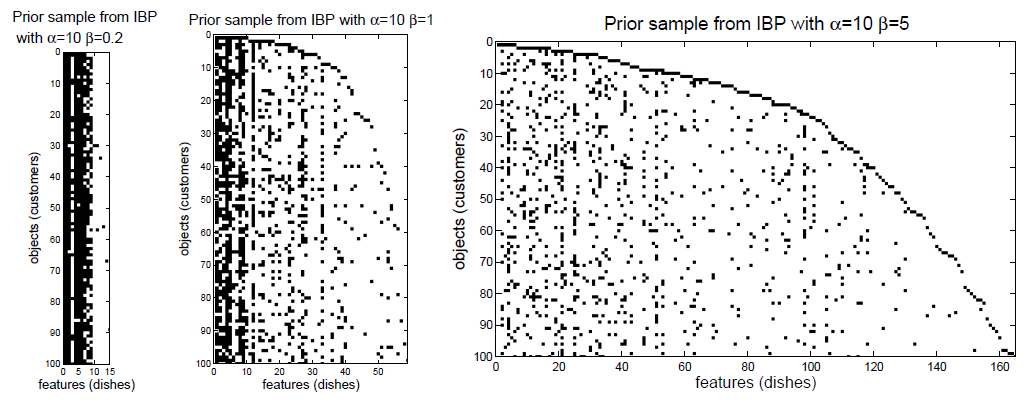
\includegraphics[scale=0.5]{img/IBP2params.png}
	\caption{Three matrices produced with the IBP.\citep{griffiths2011indian}}
\end{figure}

\subsection{Attributes with monotone preferences and $\Lambda_k$} \label{sec:lambda}

The second object of interest are the product classes $\Lambda_k$ associated with each feature. 
We need to define a distribution over the space of Cartesian products of possible $\Lambda_{ki}$ excluding the empty set. 
While there is no closed form for the distribution of $\Lambda_k$ we can define a generating process in two steps. The first step generates the set of active attributes $C_{k}$ with cardinality $c_k$ and the second step determines the set of active levels $\Lambda_{ki}$ for each active attribute.

It is possible that we want to restrict preferences such that they only increase in some attributes.
For such attribute, the active levels are restricted to be of the form $\{l,l+1,\ldots,L\}$ if the the class $\Lambda_k$ is associated with a $s_{nk}=1$, and of the form $\{1,\ldots,l-1,l\}$ if the class is associated with a $s_{nk}=0$. We denote the first case as a upper active levels, and the second as lower active levels. If a class $\Lambda_k$ has at least one active monotone attribute, we denote it by a corresponding indicator $m_k=1$, and $m_k=0$ otherwise.
Note that if several monotone attributes are active in the class, they should all be of the same type. If all the active monotone attribute are of the upper active levels type, we say that the class has a positive polarity and denote it $\rho_k=1$. conversely, if the monotone attributes are of the lower active levels type, we say that the class has a negative polarity and denote it $\rho_k=0$.

This leads us to the following generating process for drawing a $\Lambda_k$:
\begin{itemize}
	\item Draw the number of active attributes $A \sim U(1,...,L)$
	\item Draw polarity $\rho_k \sim Bernoulli(0.5)$
	\item Initialize the monotonicity indicator $m_k = 0$
	\item Draw $A$ attributes represented by the set $L^*$: 
	\item For each $i \in L^*$:
	\begin{itemize}
		\item If attribute $i$ is monotone :
		\begin{itemize}
			\item Set $m_k = 1$
			\item Draw one level $l \sim U(1,...,L_i)$
			\item If $\rho_k = 1$:
			\begin{itemize}
				\item Set level $l$ and all level above to active
			\end{itemize}
			\item If $\rho_k = 0$:
			\begin{itemize}
				\item Set level $l$ and all level below to active
			\end{itemize}
		\end{itemize}
		\item Else :
		\begin{itemize}
			\item Draw the number of active levels $a \sim U(1,...,L_i-1)$
			\item Draw $a$ level without replacement and set them to active
		\end{itemize}
	\end{itemize}
	\item For each $i \notin L^*$:
	\begin{itemize}
		\item Set all levels of attribute $i$ to active
	\end{itemize}
\end{itemize}

A more general alternative could be used for the generating process. We first draw the number of active attributes $c_k$ with a completely flexible distribution $\pi^\Lambda$ is an n-vector giving the prior distribution of number of active attributes in utility term $k$. Given the number of active attributes, the set of active attributes is given by {\em conditional} Poisson sampling from the set $\{1,\ldots,L\}$, with sample size $c_{k}$ and parameter vector $\lambda \in \mathbb{R}^L$.
The vector $\lambda$ gives the relative importance of the various attributes.
A higher weight $\lambda_i$ indicates that attribute $i$ is more likely to be active in any given utility term.
Conditional Poisson sampling guarantees that the random set $C_{k}$ has cardinality $c_{k}$ with probability one.
The normalization factor associated with conditional Poisson sampling is not known in closed form, but there is an efficient algorithm for computing it.
Given the set $C_{k}$ of active attributes, subsets $\Lambda_{ki}$, $i \in C_{k}$, are mutually independent.
For non monotone attributes, the set of active levels is obtained by Poisson sampling, truncated to assign probability zero to both the empty set and the the set containing all the possible levels. For monotone attributes, the set is drawn following the same process as in the simple case.

\subsection{Other parameters}

The other parameters $(s_{nk},\theta_{nk},\epsilon_{nkt})$ are defined conditional on $z_{nk}$. When $z_{nk}=0$, the values of all these parameters are arbitrarily set to $0$. We have to define the prior distributions of $(s_{nk},\theta_{nk},\epsilon_{nkt})$ conditional on $z_{nk}=1$:
$$ s_{nk}|\pi_k^s,z_{ik}=1 \sim \left\{ \begin{array}{cl}
0 & if \; m_k=1 \text{ and } \rho_k=1\\
1 & if \; m_k=1 \text{ and } \rho_k=0\\
Bernoulli(\pi_k^s) & \text{otherwise}\\
\end{array}\right.$$
$$ \theta_{nk}|\sigma^\theta,\alpha_\theta,z_{ik}=1 \sim Gamma(\sigma^\theta \alpha^\theta,1) $$
$$ \epsilon_{nkt}|\sigma^\theta,\alpha^\theta,z_{ik}=1 \sim Gamma((1-\sigma^\theta)\alpha^\theta,1) $$
where $(s_{nk},\theta_{nk})$ are independent across $n$ and $k$; and $\epsilon_{nkt}$ are independent across $n$,$k$ and $t$.

Note that the distribution of the value size $(\theta_{nk} + \epsilon_{nkt})$ is also Gamma with parameters $Gamma(\alpha^\theta,1)$ from the properties of a sum of Gamma distributed variables. The parameter $\alpha^\theta$ is the shape parameter of the distribution of the value size, while $\sigma^\theta$ can be interpreted as a stability parameter. 
For $\sigma^\theta$ close to one, the stable component $\theta_{nk}$ is favored and the utility functions have high serial dependence; for $\sigma^\theta$ close to zero, the variable component $\epsilon_{nkt}$ is favored and the utility function has low serial dependence.

Finally, we have to define hyperpriors on some of the hyperparameters:
$$\alpha^\theta \sim Gamma(1,1)$$
$$\sigma^\theta \sim Gamma(1,1)$$
$$ \pi_k^s \sim Beta(1,1) $$


\section{Inference}

\subsection{Likelihood and Posetrior} \label{sec:likelihood}
Conditional on the set of parameters $\psi$, there is no random term in the utility function. The likelihood becomes a degenerate function that is equal to $1$ if all the observed choices are predicted correctly and $0$ otherwise. The probability of observing the set of choices $\{x_{nt}^*\}$ is: 
$$P(\{x_{nt}^*\}|\psi) = \mathds{1}\{ \arg \max\limits_{x\in X_{nt}} u(x,\psi) = x_{nt}^*, \forall n,t \}$$

Likelihood-based inference consists in recovering the identified set of parameters such that: $$P(\{x_{nt}^*\}|\psi) = 1 $$
We can see that with the current likelihood function, if at least one choice is not maximizing utility according to the current value of $\psi$, the likelihood takes the value of $0$.

In the Bayesian framework, the target distribution is the corresponding posterior:
$$  P(\psi|\{x_{nt}^*\}) \propto P(\{x_{nt}^*\}|\psi) \cdot P(\psi),$$
where $P(\psi)$ denotes the prior density of our parameters.

\subsection{Tempering and Sequence of Distributions} 

Simulating the posterior can be quite difficult, and we simulate instead a sequence of target distributions converging to this Posterior. The functions used in the sequence are increasingly difficult to simulate. This process is known as tempering, and we achieve it by combining two methods. First, we use Data Tempering and introduce the observations one by one in the likelihood. We start with the first observation of the first individual $x_{1,1}^*$, then add the subsequent observations for this individual until all the observations are included in the likelihood. We then add the observations of the following individual, and continue until every observation of every individual are included. For the second tempering approach, we use an instrumental function that does not take a value of zero if the last observed choice is not utility maximizing with the current value of $\psi$. We call this approach $\zeta$-tempering and substitute the likelihood with the following function:  
$$Q(\{x_{nt}^*\}|\psi;\eta,\tau,\zeta) = P(\{\{x_{nt}^*\}_{t=1}^T\}_{n=1}^{\eta-1}|\psi) \cdot  P(\{x_{\eta t}^*\}_{t=1}^{\tau-1}|\psi) \cdot \zeta^{ u(x_{\eta \tau}^*,\psi) - \max_{x \in X_{\eta \tau}} u(x,\psi)},$$
where $\zeta>1$ is a constant chosen by the researcher. We can see that this instrumental function is the product of $3$ terms. The first one is the likelihood of observing the choices of individuals $1$ to $\eta-1$. The second is the likelihood of observing the $\tau-1$ first choices of individual $\eta$. The last term requires further attention. If the last observed choice is utility maximizing, this term is equal to $1$ as for the likelihood. However, it is equal to a value between $0$ and $1$ if another choice would be utility maximizing. The smaller the difference between the observed choice and the utility maximizing one, the closer the term gets to $1$. It is important to note that $Q(\{x_{nt}^*\}|\psi;\eta,\tau,\zeta) \to P(\{x_{\eta t}^*\}_{t=1}^\tau \cup \{\{x_{nt}^*\}_{t=1}^T\}_{n=1}^{\eta-1}|\psi)$ as $\zeta \to \infty$. 

The corresponding quasi-posterior distribution is defined as
$$ Q(\psi|\{x_{nt}^*\};\eta,\tau,\zeta) \propto Q(\{x_{nt}^*\}|\psi;\eta,\tau,\zeta) \cdot P(\psi) .$$

Using these tempering approaches, we can define a sequence of distributions by specifying the values $(\eta,\tau,\zeta)$ for each distribution in the sequence. We start by the distribution 
$$Q(\psi|\{x_{nt}^*\};\eta=1,\tau=1,\zeta=2) \propto 2^{ u(x_{1,1}^*,\psi) - \max_{x \in X_{1,1}} u(x,\psi)} \cdot P(\psi)$$ 
and progressively increase $\zeta$ in each subsequent distribution until $\zeta \to \infty$ and the target distribution becomes
$$ Q(\psi|\{x_{nt}^*\};\eta=1,\tau=1,\zeta \to \infty) \propto  P(\psi|\{x_{1,1}^*\}).$$

We then alternatively increase the value of $\tau$ by $1$ and progressively increase $\zeta$ from $2$ to $\infty$ until we reach the last observation $T$ for the current individual. For our application, we choose to increase $\zeta$ by a factor of $2$ with each step in the sequence. We then increase $\eta$ by one and start again alternatively increasing the value of $\tau$ by $1$ and progressively increasing $\zeta$ from $2$ to $\infty$ until we reach the last observation of the last individual $N$.

The ratio of two consecutive target distributions when increasing $\zeta$ by a factor of $a$ is equal to
$$ \frac{P(\{\{x_{nt}^*\}_{t=1}^T\}_{n=1}^{\eta-1}|\psi) \cdot  P(\{x_{\eta t}^*\}_{t=1}^{\tau-1}|\psi) \cdot (a \zeta)^{ u(x_{\eta \tau}^*,\psi) - \max_{x \in X_{\eta \tau}} u(x,\psi)}}{P(\{\{x_{nt}^*\}_{t=1}^T\}_{n=1}^{\eta-1}|\psi) \cdot  P(\{x_{\eta t}^*\}_{t=1}^{\tau-1}|\psi) \cdot \zeta^{ u(x_{\eta \tau}^*,\psi) - \max_{x \in X_{\eta \tau}} u(x,\psi)}} = a^{ u(x_{\eta \tau}^*,\psi) - \max_{x \in X_{\eta \tau}} u(x,\psi)}.$$

The ratio of two consecutive target distributions when increasing $\tau$ by $1$ and reseting $\zeta$ to $2$ is equal to:
$$ \frac{  P(\{\{x_{nt}^*\}_{t=1}^T\}_{n=1}^{\eta-1}|\psi) \cdot  P(\{x_{\eta t}^*\}_{t=1}^{\tau-1}|\psi) \cdot 2^{ u(x_{\eta \tau}^*,\psi) - \max_{x \in X_{\eta \tau}} u(x,\psi)}}{P(\{\{x_{nt}^*\}_{t=1}^T\}_{n=1}^{\eta-1}|\psi) \cdot  P(\{x_{\eta t}^*\}_{t=1}^{\tau-1}|\psi)} = 2^{ u(x_{\eta \tau}^*,\psi) - \max_{x \in X_{\eta \tau}} u(x,\psi)} $$

\subsection{Quasi-Posterior Simulation}

We propose the adaptive Sequential Monte Carlo (SMC) approach \citep{DurhamGeweke2013} as a posterior simulation strategy, for two main reasons.
First, many utility functions of the form in \eqref{e:uff} give identical predictions.
We cannot expect these functions to be close, in the sense of a practical MCMC chain passing from one to the other in a small number of steps with reasonable probability. Having many particles exploring the parameter space solves that problem.
Second, a sequential inference method is required for our tempering approach.

The sequence of target distributions is obtained by setting $\zeta=2$ for the first distribution, and by increasing $\zeta$ by a factor of $2$ at each iteration:
$$ Q(\psi|\{x_{nt}^*\},\zeta), \; \text{ for } \zeta=2,4,8,\ldots $$ 


\subsubsection{Algorithm}

The algorithm uses a population of $J$ groups of $P$ particles, each of them containing a set of realizations of all our parameters and some simulated hyperparameters that do not have a closed form posterior: $$\psi_{jp} = \left\{\alpha^\theta, \sigma^\theta, K_+,\left\{\Lambda_k, \pi^z_k, \{z_{nk},s_{nk},\theta_{nk},\{\epsilon_{nkt}\}_{t=1}^T \}_{n=1}^N \right\}_{k=1}^{K_+} \right\}.$$

The algorithm starts with an Initialization $(I)$ phase and then iterates over Correction $(C)$, Selection $(S)$ and Mutation $(M)$ phases. 

The first group of particles will be used to determine when to move from the C phase to the S phase based on Effective Sample Size (ESS). The ESS for the first group of particles will be denoted $ESS_1$. The simulated values of our first group of particles will be discarded in our analysis of the simulated posterior.  

The general structure of the algorithm is as follow:


\begin{itemize}
	\item Initialization phase: Initialize $J \times P$ particles $\{\{\psi_{jp}\}_{p=1}^P\}_{j=1}^J$
	\item For $\eta=1$ to $N$ {\it (Iterate over individuals)}
	\begin{itemize}
		\item Draw $\{z_{\eta k},s_{\eta k},\theta_{\eta k}\}$ for the newly added individual (\textit{see section \ref{sec:drawparams}})
		\item For $\tau=1$ to $T$ {\it (Iterate over observations for each individual)}
		\begin{itemize}
			\item Draw $\epsilon_{\eta k \tau}$ for the newly added observation (\textit{see section \ref{sec:drawparams}})
			\item Set $\zeta = 1$
			\item Repeat until $\zeta = \infty$:
			\begin{itemize}
				\item Correction phase: increase $\zeta$ until $ESS_1/P<0.5$ or $\zeta=\infty$ (\textit{see section \ref{sec:correction}})
				\item Selection phase: re-sample particles within each group based on weight
				\item Mutation phase: move each particle with an Metropolis-Hastings within Gibbs step using the target density $ Q(\psi_{jp}|\{x_{nt}^*\};\eta,\tau,\zeta) $
			\end{itemize}
		\end{itemize}
	\end{itemize}
\end{itemize}

The various parts of the algorithm are detailed in the following sections.

\subsubsection{Initialization phase}

Applied to every particle:

\begin{itemize}
	\item Draw $\alpha^\theta \sim Gamma(1,1)$
	\item Draw $\sigma^\theta \sim Gamma(1,1)$
	\item Set $K_+ = 0$
\end{itemize}

\subsubsection{Drawing $\{z_{\eta k},s_{\eta k},\theta_{\eta k}\}$ and  $\{\epsilon_{\eta k \tau}\} $}\label{sec:drawparams}
To draw the $z_{\eta k}$ we follow the IBP approach. As detailed in section \ref{sec:lambda}, when $\Lambda_k$ has an active monotone attribute, we set $m_k=1$. When the monotone active attributes have upper active levels (all levels above a specified level are active), we set $\rho_k=1$. When the monotone active attributes have lower active levels (all levels below a specified level are active), we set $\rho_k=0$.
\begin{itemize}
	\item For $k=1$ to $K_+$
	\begin{itemize}
		\item If $\sum_{n=1}^{\eta-1} z_{nk} > 0 $:
		\begin{itemize}
			\item Draw $z_{nk} \sim Bernoulli(\frac{\sum_{n=1}^{\eta-1} z_{nk}}{\beta^z + \eta - 1})$
			\item If $z_{nk} = 1$: 
			\begin{itemize}
				\item Draw $s_{\eta k} \sim \left\{ \begin{array}{cl}
				0 & if \; m_k=1 \text{ and } \rho_k=1\\
				1 & if \; m_k=1 \text{ and } \rho_k=0\\
				Bernoulli(\frac{1 + \sum_{n=1}^{\eta-1} s_{nk}}{2+\eta-1}) & \text{otherwise}\\
				\end{array}\right.$
				\item Draw $\theta_{\eta k} \sim Gamma(\sigma^\theta \alpha^\theta,1)$
			\end{itemize}
		\end{itemize}
		\item Else :
		\begin{itemize}
			\item Set $z_{nk}=0$
		\end{itemize}
	\end{itemize}
	\item If $K_+=0$:
	\begin{itemize}
		\item While $k^* < 1$ : Draw $k^* \sim Poisson(\frac{\alpha^z \beta^z}{\beta^z + \eta - 1})$
	\end{itemize}
	\item Else:
	\begin{itemize}
		\item Draw $k^* \sim Poisson(\frac{\alpha^z \beta^z}{\beta^z + \eta - 1})$
	\end{itemize}
	\item Set $K_+ = K_+ + k^*$
	\item For $k=K_+ - k^*$ to $K_+$
	\begin{itemize}
		\item Det $z_{\eta k} = 1$
		\item Draw $\Lambda_k$
		\item Draw $s_{\eta k} \sim \left\{ \begin{array}{cl}
		0 & if \; m_k=1 \text{ and } \rho_k=1\\
		1 & if \; m_k=1 \text{ and } \rho_k=0\\
		Bernoulli(\frac{1 + \sum_{n=1}^{\eta-1} s_{nk}}{2+\eta-1}) & \text{otherwise}\\
		\end{array}\right.$
		\item Draw $\theta_{\eta k} \sim Gamma(\sigma^\theta \alpha^\theta,1)$
	\end{itemize}
\end{itemize} 

In order to draw the $\{\epsilon_{\eta k \tau}\}$ when a new observation is added, we follow the following simple algorithm:

\begin{itemize}
	\item For $k=1$ to $K_+$
	\begin{itemize}
		\item If $z_{\eta k}=1$ : Draw $\epsilon_{\eta k \tau} \sim Gamma((1-\sigma^\theta) \alpha^\theta,1)$
	\end{itemize}
\end{itemize} 	


\subsubsection{Correction phase}\label{sec:correction}

Applied to every particle:

\begin{itemize}
\item Repeat until $ESS_1/P<0.5$ or $\zeta=\infty$:
	\begin{itemize}
		\item compute utility differences  $du_{jp} = u(x_{\eta \tau}^*,\psi_{jp}) - \max_{x \in X_{\eta \tau}} u(x,\psi_{jp})$
		\item If $\sum_p du_{1p} = 0$:
		\begin{itemize}
			\item Set $\zeta=\infty$
			\item compute weight $w_{jp} = \mathds{1}\{du_{jp}=0\}$
		\end{itemize}
		\item Else:
		\begin{itemize}
			\item Set $\zeta= 2 \cdot \zeta $
			\item compute weight $w_{jp} = w_{jp} \cdot 2^{ du_{jp}}$
		\end{itemize}
	\end{itemize}
	\item compute $ESS_1/P = \frac{(\sum_p w_{1p})^2}{\sum_p w_{1p}^2}$
\end{itemize}



\subsubsection{Selection phase}

The selection phase draws a new set of $P$ within group $j$ particles with replacement from the set of old particles using weights $w_{jp}$. For each group $j$ of particle:

\begin{itemize}
	\item For each group $j$ of particle:
	\begin{itemize}
		\item For $p'=1$ to $P$
		\begin{itemize}
			\item Draw a particle $\psi^*$ from set $\{\psi_{jp}\}_{p=1}^P$ using weights $\{w_{jp}\}_{p=1}^P$
			\item Set $\psi_{jp'} = \psi^*$
		\end{itemize}
	\end{itemize}
\end{itemize}

\subsubsection{Mutation phase}

The mutation phase do an MCMC step using Gibbs sampling and Metropolis-Hastings (MH) accept-reject algorithm.

\begin{itemize}
	\item For $n=1$ to $\eta$
	\begin{itemize}
		\item For $k=1$ to $K_+$
		\begin{itemize}
			\item If $\sum_{n' \neq n} z_{n'k} > 0 $:
			\begin{itemize}
				\item Set $\psi^* = \psi_{jp}$
				\item Draw $z^*_{nk} \sim Bernoulli(\frac{\sum_{n' \neq n} z_{n'k}}{\beta^z + \eta - 1})$
				\item If $z_{nk} = 1$: Draw $\{s^*_{nk},\theta^*_{nk},\{\epsilon^*_{nkt}\}\}$ (\textit{see below})
				\item Store new values into $\psi^*$
				\item Set $\psi_{jp} = \psi^*$ with probability $\min\{1, \frac{ Q(\{x_{nt}^*\}|\psi^*;\eta,\tau,\zeta) }{ Q(\{x_{nt}^*\}|\psi_{jp};\eta,\tau,\zeta)} \}$
			\end{itemize}
			\item Else :
			\begin{itemize}
				\item Set $z_{nk}=0$
			\end{itemize}
		\end{itemize}
		\item Draw $k^* \sim Poisson(\frac{\alpha^z \beta^z}{\beta^z + \eta - 1})$
		\item Set $K_+ = K_+ + k^*$
		\item For $k=K_+ - k^*$ to $K_+$
		\begin{itemize}
			\item Set $\psi^* = \psi_{jp}$
			\item Set $z^*_{n k} = 1$
			\item Draw $\Lambda^*_k$
			\item Draw $s^*_{n k} \sim \left\{ \begin{array}{cl}
			0 & if \; \Lambda^*_k \text{ has active upper monotone atributes}\\
			1 & if \; \Lambda^*_k \text{ has active lower monotone atributes}\\
			Bernoulli(\frac{1 + \sum_{n=1}^{\eta-1} s_{nk}}{2+\eta-1}) & \text{otherwise}\\
			\end{array}\right.$
			\item Draw $\theta^*_{n k} \sim Gamma(\sigma^\theta \alpha^\theta,1)$
			\item Store new values into $\psi^*$
			\item Set $\psi_{jp} = \psi^*$ with probability $\min\{1, \frac{ Q(\{x_{nt}^*\}|\psi^*;\eta,\tau,\zeta) }{ Q(\{x_{nt}^*\}|\psi_{jp};\eta,\tau,\zeta)} \}$
		\end{itemize}
	\end{itemize}
	
	\item Draw $\alpha^* \sim Gamma(1,1)$
	\item Draw $\sigma^* \sim Gamma(1,1)$
	\item Set $(\alpha^\theta,\sigma^\theta)=(\alpha^*,\sigma^*)$ with probability $$\min\left\{ 1 , \prod_{k}^{K_+} \prod_{n}^{\eta} \left( \frac{ 
		P_\Gamma(\theta_{nk}|\alpha^* \sigma^*,1) \prod_{t}^{T_n} P_\Gamma(\epsilon_{nkt}|\alpha^* (1-\sigma^*),1) 
	}{
		P_\Gamma(\theta_{nk}|\alpha^\theta \sigma^\theta,1) \prod_{t}^{T_n} P_\Gamma(\epsilon_{nkt}|\alpha^\theta (1-\sigma^\theta),1) 
	} \right)^{z_{nk}} \right\}$$
	where $P_\Gamma(\cdot|\alpha,\beta)$ is the PDF of the $Gamma(\alpha,\beta)$ distribution, and $T_n=\tau$ if $n=\eta$ and $T_n=T$ otherwise.
\end{itemize}


For this phase, in order to draw $\{s^*_{nk},\theta^*_{nk},\{\epsilon^*_{nkt}\}\}$, we propose the following process:

\begin{itemize}
	\item Draw $s^*_{n k} \sim \left\{ \begin{array}{cl}
	0 & if \; m^*_k=1 \text{ and } \rho^*_k=1 \\
	1 & if \; m^*_k=1 \text{ and } \rho^*_k=0 \\
	Bernoulli(\frac{1 + \sum_{n'\neq n}^{\eta} s_{nk}}{2+\eta-1}) & \text{otherwise}\\
	\end{array}\right.$
	\item Draw $\theta^*_{n k} \sim Gamma(\sigma^\theta \alpha^\theta,1)$
	\item If $n<\eta$:
	\begin{itemize}
		\item For $t=1$ to $T$:
		\begin{itemize}
			\item $\epsilon^*_{n k t} \sim Gamma((1-\sigma^\theta) \alpha^\theta,1)$
		\end{itemize} 
	\end{itemize}
	\item Else:
	\begin{itemize}
		\item For $t=1$ to $\tau$:
		\begin{itemize}
			\item $\epsilon^*_{n k t} \sim Gamma((1-\sigma^\theta) \alpha^\theta,1)$
		\end{itemize} 
	\end{itemize}
	
\end{itemize}

\bibliography{Lit-review}{}
\bibliographystyle{plain}





\end{document} 